\chapter{Preliminary implementation} % (fold)
\label{cha:framework}

In this chapter we present our preliminary implementation composed of three
modules: one front-end for the users to iteract with the system, one engine to
choose good job configurations called tuning-by-testing and one back-end to
report the new job configuration.

\section{Overview}

In figure~\ref{fig:overview} we show all components together. Fist of all, the
user creates one file containing initial knobs, this file is submitted to component
front-end which performs lexical, syntatic and semantic analysis on the file, after
it is parsed and sent to engine component. This component, as described previously,
actives the BA to choose one good job configuration until it reaches the criteria. The
result is passed to back-end component that saved in a file.

One interesting feature is the result file can be used as input for the next round
of the self-tuning, just only the user submit it as input. So the framework can work
as incremental software to improve its last result.

\begin{figure}[htbp]
	\centering
	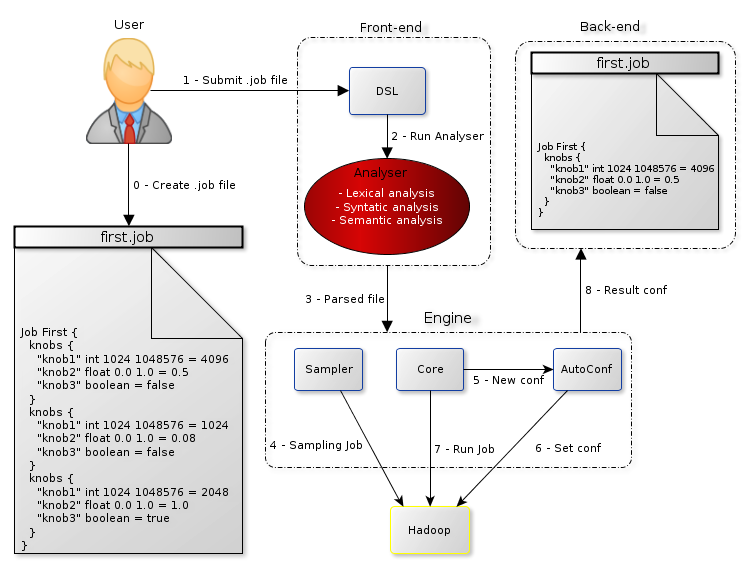
\includegraphics[width=420px,height=330px]{img/overview.png}
	\caption{Implementation overview.}\label{fig:overview}
\end{figure}

\section{Front-end}

The front-end is the DSL shown in the chapter \ref{cha:dsl}, it consists in
saying what is the job name to choose a good configuration and one or several set of
knobs with their initial values, which can be assigned with any values since the
last configuration or rule of thumbs until a random assignment.

One use case of the DSL is shown below, it contains the job name \textbf{WordCount},
its properties and several sets of knobs. The sets of knobs form the initial population
for the BA, each set of knob ({\bf knobs}) represents one individual
and one single knob corresponds one gene, any change is done on knob level.

\singlespacing
\begin{listing}[H]
\begin{minted}[mathescape,frame=lines,framesep=2mm,fontfamily=courier,fontsize=\scriptsize]{python}
Job WordCount {
    Properties {
        jarPath /tmp/test/wc/wordcount.jar
        inputHDFSDir /tmp/test/wc/input
        outputHDFSDir /tmp/test/wc/output
        samplePercent 0.2
    }
    knobs {
	    "dfs.block.size" int 1024 1048576 = 4096
	    "io.sort.spill.percent" float 0.0 1.0 = 0.5 
	    "mapred.map.tasks.speculative.execution" boolean = false
    }
    knobs {
	    "dfs.block.size" int 1024 1048576 = 1024
	    "io.sort.spill.percent" float 0.0 1.0 = 0.08
	    "mapred.map.tasks.speculative.execution" boolean = false
    }
    knobs {
	    "dfs.block.size" int 1024 1048576 = 1048576
	    "io.sort.spill.percent" float 0.0 1.0 = 1.0
	    "mapred.map.tasks.speculative.execution" boolean = true
    }
}
\end{minted}
\caption{Example of a configuration written in our proposal DSL.} 
\label{listing:usageDSL}
\end{listing}

As shown in~\ref{listing:usageDSL} there are four properties for the job: the jar path, the HDFS
input directory where are stored the input files, the HDFS output directory and the sample
percent. Also there are three initial set of knobs to test, in this example
the first set could be the last job configuration, the second the rule of thumbs
suggested by the comunity and the last one random assignment. However, the users
can be interested in testing new set of knobs that would be easy, just put a new
set of knobs to test, so this front-end covers quite use cases as the users wish.

\section{Engine}

The engine is divided in three components: the component to generate
data sample, the component to auto configure Hadoop and the core component that
choosing configurations based on the BA.

 with all configurations generated
by  that is responsible for choosing job configurations using BA.

\begin{figure}[htbp]
	\centering
	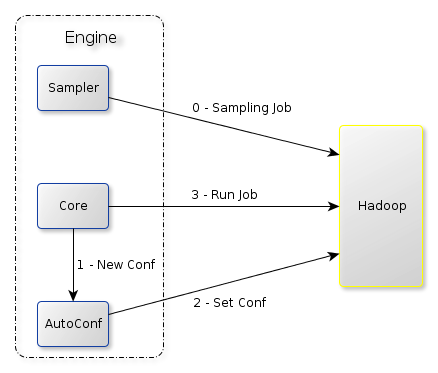
\includegraphics[width=230px,height=200px]{img/engine.png}
	\caption{Engine processing.}\label{fig:engine}
\end{figure}

\subsection{Sampler component}engine

The sampler is responsable to generate data sample, so it sends a command to hadoop
in order to run the sampling job and its output will be used by the core component,
this step is represented by the action {\it \bf 0 - Sampling Job}.

\subsection{AutoConf component}

The AutoConf is one component developed by Ramiro, E~\footnote{\href {https://github.com/erlfilho/AutoConf}}.%\textcolor{red}{colocar referência do autoconf}
It is responsable for communicate with the Hadoop and inject new job configuration,
as seen in the action {\bf 2 - Set Conf}. Despite the configurations assigned for
the user in the Hadoop configuration files, the Hadoop will use job configurations
sent for AutoConf.

\subsection{Core component}

The core component generates job configurations using the BA in order to test its performance
and evaluate the response time, it sends the action {\bf 1 - New Conf} to component AutoConf.
After assigned the configuration, the job is submited to Hadoop through the action {\bf Run Job},
then its response time is evaluated and the job configuration maybe added or not to list of good
configurations. The actions sequence {\it 1, 2 and 3} occur until the BA finishes,
i.e., until one criteria is reached.

\section{Back-end}

The back-end at the moment is is still being developed, currently the result is being saved in
one file with the same format of the input file, but it contains just the best
job configuration found by the core component.
